\documentclass[12pt]{extarticle}
\usepackage{geometry}
\geometry{
a4paper,
total={170mm,257mm},
left=20mm,
top=20mm,
headheight=12pt
}

\usepackage[parfill]{parskip} % Activate to begin paragraphs with an empty line rather than an indent
\usepackage{graphicx} % Use pdf, png, jpg, or eps§ with pdflatex; use eps in DVI mode
% TeX will automatically convert eps --> pdf in pdflatex
\graphicspath{ {./Figures/} }
\usepackage[labelfont=bf]{caption}
\usepackage{float}

\usepackage{amssymb,amsmath,amsthm}
\usepackage{commath}
\usepackage[hyphens]{url}
\usepackage[dvipsnames]{xcolor}
\usepackage[unicode=true,colorlinks=true,urlcolor=CadetBlue,citecolor=black,linkcolor=black]{hyperref}
\PassOptionsToPackage{hyphens}{url} % url is loaded by hyperref
\usepackage{authblk}
\usepackage{longtable}
\usepackage{multirow}
\usepackage{booktabs}
\usepackage{lipsum}  
\usepackage[title,page]{appendix}
\usepackage{chngcntr}
%\usepackage{endfloat}
      
%SetFonts
% newtxtext+newtxmath
\usepackage{newtxtext} %loads helv for ss, txtt for tt
\usepackage{amsmath}
\usepackage[bigdelims]{newtxmath}
\usepackage[T1]{fontenc}
\usepackage{textcomp}
%SetFonts

% less space before sections 
% \@startsection {NAME}{LEVEL}{INDENT}{BEFORESKIP}{AFTERSKIP}{STYLE} 
%            optional * [ALTHEADING]{HEADING} 
\makeatletter
 \renewcommand\section{\@startsection {section}{1}{\z@}%
     {-2.5ex \@plus -1ex \@minus -.2ex}%
     {1.3ex \@plus.2ex}%
    {\Large\bfseries}}
    
% Species names
%% Meta-Command for defining new species macros
\usepackage{xspace}

\newcommand{\species}[3]{%
  \newcommand{#1}{\gdef#1{\textit{#3}\xspace}\textit{#2}\xspace}}
  
\species{\yeast}{Saccharomyces cerevisiae}{S.~cerevisiae}
\species{\calbicans}{Candida albicans}{C.~albicans}
\species{\cneoformans}{Cryptococcus neoformans}{C.~neoformans}

% line numbers
\usepackage[displaymath, mathlines]{lineno}
\renewcommand\linenumberfont{\normalfont\small\sffamily}
\linenumbers
\modulolinenumbers[2]

% Yoav & Lee commands
\newcommand*{\tr}{^\intercal}
\let\vec\mathbf
\newcommand{\matrx}[1]{{\Big[ \stackrel{}{#1}\Big]}}
\newcommand{\diag}[1]{\mbox{diag}\matrx{#1}}
\newcommand{\goesto}{\rightarrow}
\newcommand{\dspfrac}[2]{\frac{\displaystyle #1}{\displaystyle #2} }
\newtheorem{theorem}{Theorem}
\newtheorem{corollary}{Corollary}
\newtheorem{lemma}{Lemma}
\newtheorem{remark}{Remark}
\newtheorem{result}{Result}
\renewcommand\qedsymbol{} % no square at end of proof
\newcommand{\cl}{\mathbf{L}}
\newcommand{\cj}{\mathbf{J}}
\newcommand{\ci}{I}

% Supplementary
% https://support.authorea.com/en-us/article/how-to-create-an-appendix-section-or-supplementary-information-1g25i5a/
\newcommand{\beginsupplement}{%
      	\setcounter{table}{0}
        \renewcommand{\thetable}{S\arabic{table}}%
        \setcounter{figure}{0}
        \renewcommand{\thefigure}{S\arabic{figure}}%
		\setcounter{equation}{0}
        \renewcommand{\theequation}{A\arabic{equation}}%
}

% autoref
\def\equationautorefname{Eq.}


% NatBib
\usepackage[round,colon]{natbib}

% Title page
\title{Non-Vertical Cultural Transmission, Assortment, \\and the Evolution of Cooperation}

% Authors
\renewcommand\Affilfont{\small}

\author[1]{Dor Cohen}
\author[2]{Ohad Lewin-Epstein}
\author[3]{Marcus W. Feldman}
\author[1,4,5,*]{Yoav Ram}

\affil[1]{School of Computer Science, Interdisciplinary Center Herzliya, Herzliya, Israel}
\affil[2]{School of Plant Sciences and Food Security, Tel Aviv University, Tel Aviv, Israel}
\affil[3]{Department of Biology, Stanford University, Stanford, CA}
\affil[4]{School of Zoology, Tel Aviv University, Tel Aviv, Israel}
\affil[5]{Sagol School of Neuroscience, Tel Aviv University, Tel Aviv, Israel}
\affil[*]{Corresponding author: yoav@yoavram.com}

\date{\today}

\begin{document}
\maketitle

% Abstract
\begin{abstract}
We study the cultural evolution of cooperation under vertical, horizontal, and oblique transmission.
Conditions are found for fixation and coexistence of cooperation and defection. 
We find that the evolution of cooperation is facilitated by horizontal transmission, especially when there is an association between cooperation and transmission, and that the effect of oblique transmission depends on the bias in horizontal transmission. Stable coexistence of cooperation and defection can occur. 
A spatial model is constructed and compared to results from an unstructured model.
Comparisons are drawn with Hamilton's rule and the concepts of relatedness and assortment.
% population mean fitness?
% TODO what about oblique?
\end{abstract}

\pagebreak


%%%%%%%%%%%%%%%%%%%%%%%%%%%
%%% Introduction
\section*{Introduction}
Cooperative behavior can reduce an individual's fitness and increase the fitness of its conspecifics or competitors~\citep{axelrod1981evolution}.
Nevertheless, cooperative behavior appears to occur in many non-human animals~\citep{dugatkin1997cooperation}, including primates~\citep{jaeggi2013natural},  rats~\citep{rice1962altruism}, birds~\citep{stacey1990cooperative,krams2008experimental}, and lizards~\citep{sinervo2006self}.
Evolution of cooperative behavior remains an important conundrum in evolutionary biology~\citep[Appendix]{Haldane1932book}.

Since the work of  \citet{hamilton1964genetical} and \citet{axelrod1981evolution}, theories for the evolution of cooperative and altruistic behaviors have been intertwined often under the rubric of \emph{kin selection}.
Kin selection theory posits that natural selection is more likely to favor cooperation between more closely related individuals.
The importance of \emph{relatedness} to the evolution of cooperation and altruism was demonstrated by \citet{hamilton1964genetical}, who showed that an allele that determines cooperative behavior will increase in frequency if the reproductive cost to the actor that cooperates, $c$, is less than the benefit to the recipient, $b$, times the relatedness, $r$, between the recipient and the actor.
This condition is  known as \emph{Hamilton's rule}:
\begin{equation} \label{eq:hamilton_rule}
c < b \cdot r,
\end{equation}
where the relatedness coefficient $r$ measures the probability that an allele sampled from the cooperator is identical by descent to one at the same locus in the recipient.

\citet{Eshel1982} studied a related model for the evolution of cooperative behavior.
Their model included \emph{assortative meeting}, or non-random encounters, where a fraction $m$ of individuals in the population each interact with an individual of the same phenotype, and a fraction $1-m$ interacts  with a randomly chosen individual.  
Such assortative meeting may be due, for example, to population structure or active partner choice.
In their model, cooperative behavior can evolve if\footnote{In an extended model, which allows an individual to encounter $N$ individuals before choosing a partner, the righthand side is multiplied by $E[N]$, the expected number of encounters \citep[eq.~4.6]{Eshel1982}.
} 
\citep[eq.~3.2]{Eshel1982}
\begin{equation} \label{eq:eshel1982}
c < b \cdot m \,,
\end{equation}
where $b$ and $c$ are the benefit and cost of cooperation. 
Here $m$ in inequality~\ref{eq:eshel1982} takes the role of the relatedness coefficient $r$ in inequality~\ref{eq:hamilton_rule}.

The role of assortment in the evolution of altruism was emphasized by \citet{Fletcher2009assortment}.
They found that in a \emph{public-goods} game, altruism will evolve if cooperative individuals experience more cooperation, on average, than defecting individuals, and ``thus, the evolution of altruism requires (positive) assortment between focal \emph{cooperative} players and cooperative acts in their interaction environment.''
With some change in parameters, this condition is summarized by \citep[eq.~2.3]{Fletcher2009assortment}
\begin{equation} \label{eq:fletcher2009}
c < b \cdot (p_C - p_D ) \,,
\end{equation}
where $p_C$ is the probability that a cooperator receives help, and $p_D$ is the probability that a defector receives help.\footnote{Inequality~\ref{eq:fletcher2009} generalizes inequality~\ref{eq:hamilton_rule} and inequality~\ref{eq:eshel1982} by substituting $p_C=r + p$, $p_D=p$ and $p_C=m + (1-m)p$, $p_D=(1-m)p$, respectively, where $p$ is the frequency of cooperators.}
See \citet{Bijma2010assortment} for treatment of non-public-goods games.


In this paper we study the evolution of a cooperative behavior that is subject to \emph{cultural transmission}, which allows an individual to acquire attitudes or behavioral traits from other individuals in its social group through imitation, learning, or other modes of communication \citep{cavalli1981cultural,richerson2008not}.
\citet{feldman1985gene} introduced the first model for the evolution of altruism by cultural transmission.
They demonstrated that if the fidelity of cultural transmission of altruism is $\varphi$, then the condition for evolution of altruism in the case of sib-to-sib altruism is \citep[Eq.~16]{feldman1985gene}
\begin{equation} \label{eq:feldman1985}
c < b \cdot \varphi - \frac{1-\varphi}{\varphi} \,.
\end{equation}
In inequality~\ref{eq:feldman1985}, $\varphi$ takes the role of relatedness ($r$ in inequality~\ref{eq:hamilton_rule}) or assortment ($m$ in inequality~\ref{eq:eshel1982}), but the effective benefit $b\cdot \varphi$ is  reduced by $(1-\varphi)/\varphi$. This shows that under a combination of genetic and cultural transmission, the condition for the evolutionary success of altruism entails a modification of Hamilton's rule (\ref{eq:hamilton_rule}).

Cultural transmission may be  viewed as vertical, horizontal or oblique:  vertical transmission occurs between parents and offspring, horizontal transmission occurs between individuals from the same generation, and oblique transmission occurs  to offspring from the generation to which their parents belong (i.e. from non-parental adults). 
Evolution under either of these transmission models can be be more rapid than under pure vertical transmission~\citep{cavalli1981cultural,lycett2008questions,ram2018evolution}.
Both \citet{woodcock2006significance} and \citet{lewin2017microbes} demonstrated that non-vertical transmission can help explain the evolution of cooperative behavior (the former using simulations with cultural transmission, the latter using a model where cooperation is mediated by microbes that manipulate their host's behavior.) 
Some of the analyses by \citet{lewin2017microbes} can be applied to cultural transmission, because models of cultural transmission are mathematically similar to those for transmission of infectious diseases~\citep{cavalli1981cultural}.

Here, we study cultural-evolution models of cooperation that include both vertical and non-vertical transmission. 
We investigate these models using mathematical analysis and simulations.  
In our models behavioral changes are mediated by cultural transmission that can occur specifically during social interactions.
For instance, there may be an association between the choice of partner for social interaction and the choice of partner for cultural transmission.
As another example, when an individual interacts with an individual of a different phenotype,  exposure to the latter may lead the former to  convert its phenotype.
Our results demonstrate that cultural transmission can enhance the evolution of cooperation even when genetic transmission cannot, partly because it facilitates the generation of assortment \citep{Fletcher2009assortment}, and partly because non-vertical transmission can diminish the effect of natural selection \citep{ram2018evolution}.
This further emphasizes that treatment of cooperation as a cultural trait, rather than a genetic one, can lead to a broader understanding of its evolutionary dynamics.


%%%%%%%%%%%%%%%%%%%%%%%%%%%
% Models
\section*{Models}

Consider a large population whose members can be one of two phenotypes: $\phi=A$ for cooperators or $\phi=B$ for defectors.
An offspring inherits its phenotype from its parent via vertical transmission with probability $v$ or from a random individual in the parental population via oblique transmission with probability $(1-v)$. 
Following~\citet{ram2018evolution}, given that the parent phenotype is $\phi$ and assuming uni-parental inheritance, % TODO cite Zefferman Behav Ecol 2016
the conditional probability that the phenotype $\phi'$ of the offspring is $A$ is 

\begin{equation} \label{eq:vertical_oblique_transmission}
P(\phi'=A \mid \phi) = \begin{cases}
v + (1-v)p, & \text{if } \phi=A \\
(1-v)p, & \text{if } \phi=B
\end{cases},
\end{equation}
where $p=P(\phi=A)$ is the frequency of $A$ among all adults in the parental generation.  

Not all adults become parents due to natural selection, and we denote the frequency of phenotype $A$ among parents by $\tilde{p}$.
Therefore, the frequency $\hat{p}$ of  phenotype $A$ among juveniles (after selection and vertical and oblique transmission) is

\begin{equation}\label{eq:horizontal}
\begin{aligned}
\hat{p} =
& \tilde{p} [v + (1-v)p] + (1-\tilde{p}) [(1-v)p] = \\
& v \tilde{p} + (1-v) p \;.
\end{aligned}
\end{equation}

Individuals are assumed to interact according to a \emph{prisoner's dilemma}.
Specifically, individuals interact in pairs; a cooperator suffers a fitness cost $0<c<1$, and its partner gains a fitness benefit $b$, where we assume $c<b$. \autoref{table:prisoner_payoff} shows the payoff matrix, i.e. the fitness of an individual with phenotype $\phi_1$ when interacting with a partner of phenotype $\phi_2$.

Social interactions occur randomly:
two juvenile individuals with phenotype $A$ interact with probability $\hat{p}^2$, two juveniles with phenotype $B$ interact with probability $(1-\hat{p})^2$, and two juveniles with different phenotypes interact with probability $2\hat{p}(1-\hat{p})$. 

Horizontal cultural transmission occurs between pairs of individuals from the same generation. 
It occurs between socially interacting partners with probability $\alpha$, or between a random pair with probability $1-\alpha$ (see~\autoref{fig:horizontal}).
%The social association $\alpha$ is therefore the fraction of population that receives (horizontal transmission) from the social interaction partner, and $1-\alpha$ receives randomly.
However, horizontal transmission is not always successful, as one partner may reject the other's phenotype. The probability for successful horizontal transmission of phenotypes $A$ and $B$ are $T_A$ and $T_B$, respectively (\autoref{table:interactions}).

Therefore, the frequency $p'$ of phenotype $A$ among adults in the next generation, after horizontal transmission, is 
\begin{equation}\label{eq:nextgen_adults}
\begin{aligned}
p' = 
& \hat{p}^2 \big[\alpha + (1-\alpha)\big(\hat{p} + (1-\hat{p})(1-T_B)\big)\big] + \\
& \hat{p}(1-\hat{p}) \big[\alpha(1-T_B) + (1-\alpha)\big(\hat{p} + (1-\hat{p})(1-T_B)\big)\big] + \\
& (1-\hat{p})\hat{p} \big[\alpha T_A + (1-\alpha) \hat{p} T_A \big] + \\
& (1-\hat{p})^2 \big[(1-\alpha) \hat{p} T_A \big] \;,
\end{aligned}
\end{equation}
which simplifies to
\begin{equation}\label{eq:nextgen_adults_slimpify}
p' = \hat{p}^2(T_B-T_A) + \hat{p}(1+T_A-T_B) \;.
\end{equation}

The frequency of $A$ among parents (i.e. after selection) follows a similar dynamic, but also includes the effect of natural selection, and is therefore
\begin{equation}\label{eq:nextgen_parents}
\begin{aligned}
\bar{w} \tilde{p}' =
& \hat{p}^2 (1+b-c) \big[\alpha + (1-\alpha)\big(\hat{p} + (1-\hat{p})(1-T_B)\big)\big] + \\
& \hat{p}(1-\hat{p}) (1-c) \big[\alpha(1-T_B) + (1-\alpha)\big(\hat{p} + (1-\hat{p})(1-T_B)\big)\big] + \\
& (1-\hat{p})\hat{p} (1+b) \big[\alpha T_A + (1-\alpha) \hat{p} T_A \big] + \\
& (1-\hat{p})^2 \big[(1-\alpha) \hat{p} T_A \big] \;,
\end{aligned}
\end{equation}
where fitness values are taken from \autoref{table:prisoner_payoff} and \autoref{table:interactions}, and the population mean fitness is
\begin{equation} \label{eq:mean_fitness}
\bar{w} =  1 + \hat{p}(b-c).
\end{equation}

\autoref{eq:nextgen_parents} can be simplified to
\begin{equation}\label{eq:nextgen_parents_simplified}
\begin{aligned}
\bar{w} \tilde{p}' =
& \hat{p}^2 (1+b-c) \big[1-(1-\hat{p})(1-\alpha)T_B)\big] + \\
& \hat{p}(1-\hat{p}) (1-c) \big[\hat{p}(1-\alpha)T_B+1-T_B \big] + \\
& (1-\hat{p})\hat{p} (1+b) \big[\hat{p}(1-\alpha) + \alpha \big] T_A + \\
& (1-\hat{p})^2 \hat{p} (1-\alpha) T_A \;.
\end{aligned}
\end{equation}
%where $\hat{p}=v\tilde{p}+(1-v)p$.

Finally, we find an equation for the frequency of phenotype $A$ among juveniles in the next generation $\hat{p}'$ as a function of the frequency in the current generation.
Starting from \autoref{eq:horizontal}, we substitute \autoref{eq:nextgen_adults_slimpify} for $p'$ and  \autoref{eq:nextgen_parents_simplified} for $\tilde{p}'$.
We therefore have
\begin{equation} \label{eq:nextgen_juveniles}
\begin{aligned}
\hat{p}' =
& \frac{v}{\bar{w}}\Big[\hat{p}^2(1+b-c)\Big[1-(1-\hat{p})(1-\alpha)T_B)\Big]\Big] + \\
& \frac{v}{\bar{w}}\Big[ \hat{p}(1-\hat{p})(1-c)\big( \hat{p}(1-\alpha)T_B + 1 - T_B \big) \Big] + \\
& \frac{v}{\bar{w}}\Big[ \hat{p}(1-\hat{p})(1+b)\big(\hat{p}(1-\alpha) + \alpha \big) T_A \Big] + \\
& \frac{v}{\bar{w}}(1-\hat{p})^2\hat{p}(1-\alpha)T_A + \\
& (1-v)\hat{p}^2(T_B-T_A) + (1-v)\hat{p}(1+T_A-T_B) \;,
\end{aligned}
\end{equation}
where $\bar{w} = 1 + \hat{p}(b-c)$. 

\autoref{table:vars_params} summarizes the model variables and parameters.


%%%%%%%%%%%%%%%%%%%%%%%%%%%
%%% Results
\section*{Results}

In the following sections, we determine the equilibria of the model, namely, solutions of $\hat{p}' = \hat{p}$, and analyze their local stability.
We then analyze the evolution of a modifier of social association.
Finally, we demonstrate the application of the conditions derived in the previous sections to predict the outcomes of stochastic simulations in a structured population.

\subsection*{Equilibria and Stability}

To determine the equilibria in our model, we analyze the fixed points of \autoref{eq:nextgen_juveniles}.
We define $f(\hat{p}) = \bar{w}(\hat{p}' - \hat{p})$.
Using \emph{SymPy} \citep{Meurer2017}, a Python library for symbolic mathematics,  this simplifies to
\begin{equation} \label{eq:general_case_polynomial}
  f(\hat{p}) = \bar{w}(\hat{p}'-\hat{p}) =
  \beta_1 \hat{p}^3 + \beta_2 \hat{p}^2 + \beta_3 \hat{p},
\end{equation}
where 
\begin{equation} \label{eq:polynomial_coefficients}
\begin{aligned}
\beta_1 &= \big[c(1-v) - b (1-\alpha v)\big] (T_A-T_B) , \\
\beta_2 &= -\beta_1 -\beta_3 ,  \\
\beta_3 &= \alpha bvT_A - cv(1-T_B) + (T_A-T_B) .
\end{aligned}
\end{equation}

If $T=T_A=T_B$ then $\beta_1=0$ and $\beta_3=-\beta_2=\alpha b vT -cv(1-T)$. 
Thus, $f(\hat{p})$ becomes a quadratic polynomial,
\begin{equation} \label{eq:equal_horizontal_transmission}
  f(\hat{p}) = \hat{p}(1-\hat{p})\big[\alpha bvT - cv(1-T)\big].
\end{equation}
Clearly the only two equilibria are the fixations  $\hat{p} =  0$ and $\hat{p} = 1$.
These equilibria are locally stable if $f'(\hat{p})<0$ near the equilibrium (see Appendix~\autoref{sec:appendixA}), where
$f'(\hat{p})=(1-2\hat{p})\big[\alpha bvT - cv(1-T)\big]$, so that
\begin{equation} \label{eq:derivative_of_phattag-phat}
\begin{aligned}
	f'(0) &=	\alpha bvT - cv(1-T), \\
	f'(1) &=	-\alpha bvT + cv(1-T).
\end{aligned}
\end{equation}
%Therefore with symmetric horizontal transmission ($T_A=T_B$), fixation of the cooperative phenotype ($\hat{p}=1$) occurs under the same condition as Corollary \ref{corollary:equal_transmission}, namely inequality~\ref{eq:equal_transmission}.


In the general case where $T_A \neq T_B$, the coefficient $\beta_1$ is not necessarily zero, and $f(\hat{p})$ is a cubic polynomial.
Therefore, three equilibria may exist, two of which are
$\hat{p} = 0 $ and $\hat{p} = 1$, and the third is
\begin{equation} \label{eq:general_equilibrium}
  \hat{p}^* =  
  \frac{\beta_3}{\beta_1}.
\end{equation}

Note that the sign of the  cubic (Eq.\ \ref{eq:general_case_polynomial}) at positive (negative) infinity is equal (opposite) to the sign of $\beta_1$. 
If $T_A>T_B$, then 
\begin{equation} \label{eq:beta1}
   \beta_1 < [c(1-\alpha v) - b(1-\alpha v)] (T_A-T_B) 
   = (1-\alpha v)(c-b)(T_A-T_B) < 0 ,
 \end{equation}
since $c<b$ and $\alpha v < 1$. Hence the signs of the cubic at positive and negative infinity are negative and positive, respectively.
First, if $\beta_3<\beta_1$ then 
$1<\hat{p}^*$ and therefore $f'(0)<0$ and $f'(1)>0$; that is, fixation of the defector phenotype $B$ is the only locally stable legitimate (i.e. between 0 and 1) equilibrium.
Second, if $\beta_1<\beta_3<0$ then 
$0<\hat{p}^*<1$ and therefore $f'(0)<0$ and $f'(1)<0$ so that both fixations are locally stable and $\hat{p}^*$ separates the domains of attraction.
Third, if $0<\beta_3$ then 
$\hat{p}^*<0$ and therefore $f'(0)>0$ and $f'(1)<0$; that is, fixation of the cooperator phenotype $A$ is the only locally stable legitimate equilibrium.

Similarly, if $T_A<T_B$, then
\begin{equation} \label{eq:beta1_rev}
   \beta_1 > [c(1-\alpha v) - b(1-\alpha v)] (T_A-T_B) 
   = (1-\alpha v)(c-b)(T_A-T_B) > 0,
 \end{equation}
since $c<b$ and $\alpha v < 1$, and the signs of the cubic at positive and negative infinity are positive and negative, respectively. 
First, if $\beta_3<0$ then $\hat{p}^*<0$ and therefore $f'(0)<0$ and $f'(1)>0$; that is, fixation of the defector phenotype $A$ is the only locally stable legitimate equilibrium.
Second, if $0<\beta_3<\beta_1$ then $0<\hat{p}^*<1$ and therefore $f'(0)>0$ and $f'(1)>0$; that is, both fixations are locally unstable and $\hat{p}^*$ is a stable polymorphic equilibrium.
Third, if $\beta_1<\beta_3$ then $\hat{p}^*>1$ and therefore $f'(0)>0$ and $f'(1)<0$, and fixation of the cooperator phenotype $A$ is the only locally stable legitimate equilibrium.

We define the \emph{cost boundaries}, $\hat\gamma_1$ and $\hat\gamma_2$,
\begin{equation} \label{eq:cost_boundaries}
\begin{aligned}
\hat\gamma_1 = \frac{b v \alpha T_A + (T_A - T_B)}{v(1-T_B)}, \quad
\hat\gamma_2 = \frac{b v \alpha T_B + (1+b) (T_A - T_B)}{v(1-T_B) + (1-v)(T_A-T_B)},
\end{aligned}
\end{equation}
and the \emph{vertical transmission threshold}, $\hat v$,
\begin{equation} \label{eq:v_threshold}
\hat v = \frac{T_B - T_A}{1-T_A} \,.
\end{equation}

First, assume $T_A<T_B$.
$\beta_3<0$ requires $\hat\gamma_1<c$,
and for $\beta_3<\beta_1$ we need $c\big[v(1-T_B) + (1-v)(T_A-T_B)\big] > bv\alpha T_B + (1+b)(T_A-T_B)$.
Note that the expression in the square brackets is positive if and only if $v > \hat v$.
Thus, for $\beta_3<\beta_1$ we need $v > \hat v$ and $\hat\gamma_2 < c$ or $v < \hat v$ and $c < \hat\gamma_2$,
and for $0<\beta_3<\beta_1$ we need $v > \hat v$ and $\hat\gamma_2 < c < \hat\gamma_1$, or $v < \hat v$ and $c < \min(\hat\gamma_1, \hat\gamma_2)$. For $\beta_1<\beta_3$ we need $v > \hat v$ and $c<\hat\gamma_2$ or $v < \hat v$ and $\hat\gamma_2<c$.
However, some of these conditions cannot be met, since $v < \hat v$ implies $c<1<\hat\gamma_2$.

Second, when $T_A>T_B$
$\beta_3>0$ requires $\hat\gamma_1 > c$. 
For $\beta_1<\beta_3$ we need $c\big[v(1-T_B) + (1-v)(T_A-T_B)\big] < bv\alpha T_B + (1+b)(T_A-T_B)$.
Thus for $\beta_1<\beta_3$ we need $v > \hat v$ and $c < \hat\gamma_2 $ or $v < \hat v$ and $c > \hat\gamma_2$.
But $\hat{v}<0$ when $T_A > T_B$, and therefore we have $\beta_1<\beta_3$ if $c < \hat\gamma_2$. Similarly, we have $\beta_3<\beta_1$ if $c > \hat{\gamma_2}$.

The following result summarizes the possible outcomes of the model (\autoref{eq:nextgen_juveniles}).
\\

\begin{result}[Equilibria and stability] \label{result:vert_obli_hori}
With vertical, horizontal, and oblique transmission, the cultural evolution of a cooperator phenotype will follow one of the following scenarios depending on the cost boundaries $\hat\gamma_1$ and $\hat\gamma_2$ and the vertical transmission threshold $\hat v$ (Eqs.~\ref{eq:cost_boundaries}-\ref{eq:v_threshold}) :

% in beta
%\begin{enumerate}
%\item \emph{Fixation of cooperation}: 
%	if \emph{(i)} $T=T_A=T_B$ and $c < b\cdot \frac{\alpha T}{1-T}$; or
%	if \emph{(ii)} $T_A>T_B$ and $0<\beta_3$; or 
%	if \emph{(iii)} $T_A<T_B$ and $\beta_1<\beta_3$.
%\item \emph{Fixation of the defection}: 
%	if \emph{(iv)}  $T=T_A=T_B$ and $c > b\cdot \frac{\alpha T}{1-T}$; or 
%	if \emph{(v)} $T_A>T_B$ and $\beta_3<\beta_1<0$; or 
%	if \emph{(vi)} $T_A<T_B$ and $\beta_3<0$.
%\item \emph{Coexistence of both phenotypes at $\hat{p}^*$}: 
%	if \emph{(vii)} $T_A < T_B$ and $0<\beta_3<\beta_1$.
%\item \emph{Fixation of either phenotype depending on initial frequency}:
%	if \emph{(viii)}  $T_A>T_B$ and $\beta_1<\beta_3<0$.
%\end{enumerate}

% in gamma
\begin{enumerate}
\item \emph{Fixation of cooperation}: 
	if \emph{(i)} $T_A \ge T_B$ and $c < \hat\gamma_1$; or 
	if \emph{(ii)} $T_A < T_B$ and $v>\hat v$ and $c < \hat\gamma_2$.
\item \emph{Fixation of defection}: 
    if \emph{(iii)} $T_A \ge T_B$ and $\hat\gamma_2 < c$; or 
	if \emph{(iv)} $T_A < T_B$ and $\hat\gamma_1 < c$.
\item \emph{Stable coexistence}: 
    if \emph{(v)} $T_A < T_B$ and $v<\hat{v}$ and $c < \hat\gamma_1$; or 
    if \emph{(vi)} $T_A < T_B$ and $v>\hat{v}$ and $\hat\gamma_2 < c < \hat\gamma_1$.
\item \emph{Unstable coexistence}:
    if \emph{(vii)} $T_A > T_B$ and $\hat\gamma_1 < c < \hat\gamma_2$.
\end{enumerate}

\end{result}
These conditions are illustrated in \autoref{fig:result3}ab.

Much of the literature on evolution of cooperation focuses on conditions for  initially rare cooperative phenotype to invade a population of defectors.
The next remarks deal with such conditions. The first introduces a condition on the cost of cooperation, $c$, and the second on the social association, $\alpha$.
\\

\begin{remark}[Condition for cooperation to increase from rarity: cost of cooperation]
\label{corollary:rarity}
If the initial frequency of cooperation is very close to zero, $\hat{p}_0 \approx 0$, then its frequency will increase if 
\begin{equation} \label{eq:unequal_transmission_from_rarity_general_case}
c < \hat\gamma_1 = \frac{b v \alpha T_A + (T_A - T_B)}{v(1-T_B)} \;.
\end{equation} 
\end{remark}

This condition merges the conditions for fixation of cooperation and for stable coexistence, which both lead to the instability of $\hat{p}=0$, the fixation of defection. In general, this condition cannot be formulated in the form of Hamilton's rule due to the horizontal transmission bias $T_A-T_B$.

Importantly, increasing social association $\alpha$ increases the boundary cost ($\partial \hat\gamma_1 / \partial \alpha > 0$), making it easier for cooperation to increase from rarity.
Similarly, increasing the horizontal transmission of cooperation, $T_A$, increases the boundary ($\partial \hat\gamma_1 / \partial T_A > 0$), facilitating the evolution of cooperation.
However, increasing the horizontal transmission of defection, $T_B$, can increase or decrease the cost boundary, but it increases the cost boundary when it is already above one ($c<1<\hat\gamma_1$): $\partial\gamma_1/\partial T_B$ is positive when $T_A > \frac{1}{1+\alpha b v}$, which gives $\hat\gamma_1>1/v$. 
Therefore, increasing $T_B$ decreases the cost boundary and limits the evolution of cooperation, but only if $T_A < \frac{1}{1+\alpha b v}$.

Increasing the vertical transmission $v$ can either increase or decrease the boundary, depending on the horizontal transmission bias, $T_A-T_B$, because $\text{sign}(\partial \hat\gamma_1 / \partial v) = -\text{sign}(T_A-T_B)$.
When $T_A<T_B$ we get $\partial \hat\gamma_1 / \partial v >0$ and therefore, as the vertical transmission increases the cost boundary increases, making it easier for cooperation to evolve from rarity. 
In contrast, when $T_A > T_B$ we get $\partial \hat\gamma_1 / \partial v <0$ and therefore, as the vertical transmission increases the cost boundary decreases making it harder for cooperation to evolve from rarity.

When there is no horizontal transmission bias, $T_A=T_B$, the next remark applies.
\\

\begin{remark}[Symmetric horizontal transmission] 
\label{corollary:equal_transmission}
If $T=T_A=T_B$, then cooperation will take over the population from any initial frequency if
\begin{equation}
\label{eq:equal_transmission}
c < b v \cdot \frac{\alpha T}{1-T} \;.
\end{equation}
\end{remark}
This condition is obtained by setting $T=T_A=T_B$ in inequality \ref{eq:unequal_transmission_from_rarity_general_case} and can be interpreted as a version of Hamilton's rule  ($c<b\cdot r$, inequality~\ref{eq:hamilton_rule}) or as a version of inequality~\ref{eq:fletcher2009}, where $v \alpha T/(1-T)$ can be regarded as the \emph{effective relatedness} or \emph{effective assortment}, respectively.
\autoref{fig:results}a illustrates this condition for $v=1$. Note that the right-hand side equals $\hat\gamma_1$ when $T=T_A=T_B$.

%In Corollary~\autoref{corollary:intermediate_association}, we examined the effect of social association on evolution of cooperation in the case of perfect vertical transmission ($v=1$).
%A more general case can be stated for $0 < v \leq 1$.
In the next remarks we examine the effect of social association on the evolution of cooperation.
\\

\begin{remark}[No social association]
\label{corollary:alpha0}
Without social association ($\alpha=0$), cooperation can increase from rarity, and go to fixation, if there is horizontal transmission bias for cooperation, $T_A>T_B$, and
\begin{equation}
\label{eq:vert_hori_alpha0}
c < \frac{T_A - T_B}{v(1-T_B)} \;.
\end{equation}
\end{remark}

\autoref{fig:result2}a illustrates these conditions, which are obtained by setting $\alpha=0$ in Eqs.\ \ref{eq:unequal_transmission_from_rarity_general_case} and \ref{eq:cost_boundaries}.
Importantly, the benefit of cooperation, $b$, does not affect the evolution of cooperation in the absence of social association. The outcome is determined only by  cultural transmission.
\\


\begin{remark}[Perfect social association]
\label{corollary:alpha1}
With perfect social association ($\alpha=1$), cooperation will increase from rarity if
\begin{equation}\label{eq:vert_hori_alpha1}
c < \frac{b v T_A + (T_A - T_B)}{v(1-T_B)} \;.
\end{equation}
\end{remark}
This condition is obtained by setting $\alpha=1$ in Eqs.\ \ref{eq:unequal_transmission_from_rarity_general_case} and \ref{eq:cost_boundaries}.

Moreover, without oblique transmission, $v=1$, the only equilibria are the fixation states, $\tilde{p}=0$ and $\tilde{p}=1$, and cooperation will evolve from any initial frequency (i.e., $\tilde{p}'>\tilde{p}$) if inequality \ref{eq:vert_hori_alpha1} applies.
This is similar to case of microbe-associated cooperation studied by \citet{lewin2017microbes}, and therefore when $v=1$, this remark is equivalent to their eq.~1.

Given the previous two remarks for no association and perfect association ($\alpha=0$ and $\alpha=1$), it is interesting to examine the general effect of social association on the evolution of cooperation.
Consider the \emph{social association boundaries}, $\hat{a}_1$ and $\hat{a}_2$,
\begin{equation}\begin{aligned}\label{eq:boundries_assortative_meeting_general_case}
  \hat{a}_1 = \frac{c\cdot v(1-T_A) -(T_A-T_B)(1+b-c)}{b\cdot v \cdot T_B}, \quad
  \hat{a}_2 = \frac{c\cdot v(1-T_B)-(T_A-T_B)}{b\cdot v\cdot T_A} \;.
\end{aligned}\end{equation}
Then the following applies.
\\

\begin{remark}[Condition for cooperation to increase from rarity: social association]
\label{corollary:intermediate_association_res3}
Cooperation will increase from rarity if social association is high enough, specifically if $\hat a_2 < \alpha$.
\end{remark}
\autoref{fig:result3}cd illustrates this condition.
\autoref{fig:result2}c demonstrates these conditions.
With horizontal transmission bias for cooperation ($T_A>T_B$), cooperation can fix from any initial frequency if $a_2<\alpha$ (green area in positive x-axis). 
With horizontal bias favoring defection ($T_A<T_B$), cooperation can fix from any frequency if social association is high, $a_1<\alpha$ (green area with $T_A<T_B$), and can also increase when rare and reach stable coexistence with defection if social association is intermediate, $a_2<\alpha$ (yellow area).
Without horizontal bias ($T_A=T_B$) fixation of cooperation occurs if social association is high enough, $\frac{c}{b} \cdot \frac{1-T}{T} < \alpha$ (inequality~\ref{eq:equal_transmission}; in this case $a_1=a_2$).

Interestingly, the effect of vertical transmission on this condition depends on the horizontal transmission bias, $\partial \hat a_2 / \partial v = b T_A (T_A-T_B)$. 
That is, with horizontal bias for cooperation, $T_A>T_B$, the boundary increases with the rate of vertical transmission, impeding the evolution of cooperation.
In contrast, with horizontal bias for defection, $T_A<T_B$, the boundary decreases with the rate of vertical transmission, facilitating the evolution of cooperation. 

These effects of vertical and oblique transmission are demonstrated in \autoref{fig:result3}cd. 
The next remarks further inspect the roles of vertical and oblique transmission in the evolution of cooperation.
\\

\begin{remark}[Necessary condition for fixation of cooperation: vertical transmission rate]
\label{corollary:vhat}
  Fixation of cooperation is possible only if the vertical transmission rate is high enough,
  \begin{equation} \label{eq:fixation_of_cooperation_vertical_transmission_condition}
    \begin{aligned}
      v>\hat{v} = \frac{T_B - T_A}{1-T_A} \;.
    \end{aligned}
    \end{equation} 
\end{remark}
%Note that $\sigma \frac{\partial \gamma_1}{\partial v} = \sigma (T_B-T_A)$ and $\sigma \frac{\partial \hat\gamma_2}{\partial v} = \sigma (T_A-T_B)(b \alpha T_B - (1+b)(1-T_A))$
This condition does not guarantee fixation of cooperation. Rather, if this condition does not apply then cooperation cannot fix.
If horizontal transmission is biased for cooperation, $T_A>T_B$, cooperation can fix with any vertical transmission rate (because $\hat{v}<0$).
In contrast, if horizontal transmission is biased for defection, $T_A<T_B$,  cooperation can fix only if the vertical transmission rate is high enough~(\autoref{eq:fixation_of_cooperation_vertical_transmission_condition}): in this case oblique transmission can prevent fixation of cooperation (see \autoref{fig:result3}bd).

With only oblique and horizontal transmission, i.e. $v = 0$, Eq.\ \ref{eq:horizontal} becomes $\hat{p}=p$ and Eq.\ \ref{eq:nextgen_adults_slimpify} becomes 
\begin{equation}  \label{eq:nextgen_parents_oblique_only}
p' = p^2 (T_B-T_A) + p (1+T_A-T_B) \;,
\end{equation}
which gives the following result.\\

\begin{remark}[Condition for global fixation of cooperation: oblique and horizontal transmission] \label{result:obli_hori}
Without vertical transmission ($v=0$), the frequency of the cooperator phenotype among adults increases every generation, $p'>p$ if there is a horizontal transmission bias in favor of cooperation, namely
\begin{equation} \label{eq:oblique_only_result}
T_A > T_B \;.
\end{equation}
\end{remark}

That is, in the absence of vertical transmission, selection plays no role in the evolution of cooperation (i.e. $b$ and $c$ are missing from \autoref{eq:nextgen_parents_oblique_only}).
The dynamics are determined solely by differential horizontal transmission of the two phenotypes, namely, the relative tendency of each phenotype to be horizontally transmitted to peers (see~{\autoref{fig:results}c).
Note that without bias in horizontal transmission, $T_A = T_B$, phenotype frequencies are static, $p'=p$.

Finally, the last remark focuses on the coexistence of cooperation and defection.
\\

\begin{remark}[Coexistence of cooperation and defection]
Cooperation and defection can coexist at frequencies $\tilde{p}^*$ and $1-\tilde{p}^*$ (\autoref{eq:general_equilibrium}). 
When it occurs, the coexistence is stable if there is horizontal transmission bias for defection, $T_A<T_B$, and unstable if there is horizontal bias for cooperation, $T_A>T_B$.
\end{remark}

% TODO - revise the next paragraph
If there is horizontal transmission bias for defection, $T_A<T_B$, and the cost of cooperation is intermediate, $\gamma_2 < c < \gamma_1$; see yellow area in \autoref{fig:result2}b.
When unstable coexistence occurs, phenotype $A$ will fix if its initial frequency is $p>\tilde{p}^*$, and phenotype $B$ will fix if its initial frequency is $1-p>1-\tilde{p}^*$; this occurs when there is horizontal transmission bias for cooperation, $T_A>T_B$, and the cost is intermediate, $\gamma_1 < c < \gamma_2$.
\autoref{fig:coexistence_recursive}a shows the mapping $\tilde p \to \tilde p'$; see blue areas in \autoref{fig:result2}a and \autoref{fig:result2}b.

% TODO - consider adding v=1 case?

%%%%%%%%%%%%%%%%%%%%%%%%%%%%%%%%%%%%%%%%%%%%%%%%
\subsection*{Population Structure}

Social association may also emerge from a population's structure.
Consider a  population colonizing a 2D grid of size 100-by-100, where each site is inhabited by one individual, similarly to \citet{lewin2020rockpaperscissors}.
Each individual is characterized by its phenotype: either cooperator, $A$, or defector, $B$.
Initially, each site in the grid is randomly colonized with either a cooperator or a defector, with equal probability.
%In each generation individuals interact with their neighbors, i.e. individuals that inhabit adjacent sites, in a prisoner's dilemma game (\autoref{table:prisoner_payoff}) and in horizontal cultural transmission (\autoref{fig:horizontal}).
%As before, $T_A$ and $T_B$ are the probabilities of transmitting phenotypes $A$ and $B$ during horizontal transmission.
In each generation, half of the individuals are randomly chosen to "initiate" interactions.
Initiators then interact with a random neighbor (i.e. individual in an adjacent site) in a prisoners' dilemma game (\autoref{table:prisoner_payoff}) and a random neighbor (with replacement) in horizontal cultural transmission (\autoref{fig:horizontal}).
The expected number of each of these interactions per individual per generation is one.
The effective social association $\alpha$ in this model is the probability that the same neighbor is picked for both interactions, or $\alpha=1/m$, where $m$ is the number of neighbors.
On an infinite grid, $m=8$, but on a finite grid $m$ can be lower in edge neighborhoods close to the grid border.
As before, $T_A$ and $T_B$ are the probability to successfully transmitting phenotypes $A$ and $B$ during horizontal transmission, respectively.

The order the interactions across the grid at each generation is random.
After all interactions take place, individual fitness is determined by
$w = 1 + b \cdot n_b - c \cdot n_c$,
where $n_b$ is the number interactions of that individual with cooperative neighbors, and $n_c$ is the total number of interactions that that individual  had ($n_b \le n_c$).
Then a new generation is generated, and sites can be settled by offspring of any parent, not just neighbor parents. Thus, selection is global, rather than local, in accordance with our deterministic model.
The parent is randomly drawn with probability proportional to its fitness, divided by the average fitness of all potential parents.
Offspring then have the same phenotype as their parents ($v=1$).

\autoref{fig:spatial} shows that the highest cost of cooperation ($c$) that permits the evolution of cooperation in simulations of the spatial model agrees with the conditions derived in Result~2.
An example for stable coexistence is shown in \autoref{fig:spatial_fluctuations}.
Simulating a spatial model with local selection (i.e. sites can only be settled by offspring of neighbor parents) had only a minor effect on the agreement with Result~2 (\autoref{fig:spatial_local_selection}).

This comparison between the deterministic well-mixed model and the stochastic spatial model demonstrates that the derived conditions can be useful for predicting the dynamics of complex scenarios. 
Moreover, our spatial model shows how social association ($\alpha$) can emerge from local interactions between individuals in a structured population.


%%%%%%%%%%%%%%%%%%%%%%%%%%%
% Discussion
\section*{Discussion}
We studied the evolution of cooperation under non-vertical transmission using deterministic discrete-time evolutionary models with fitnesses in the form of payoffs from a prisoner's dilemma game. 
Under oblique and horizontal cultural transmission, horizontal transmission bias in favor of the cooperative phenotype was found to be necessary and sufficient for evolution of cooperation (Result~\autoref{result:obli_hori}).
Under a combination of vertical, oblique, and horizontal transmission, cooperation or defection can either fix or coexist at a stable polymorphism, depending on the relationship between the cost and benefit of cooperation, the horizontal bias, and the association between cooperation and transmission (Results~\autoref{result:vert_hori} and~\autoref{result:vert_obli_hori}).
Importantly, cooperation can increase from rarity (i.e. invade a population of defectors) if and only if (inequality~\ref{eq:unequal_transmission_from_rarity_general_case}),
\begin{equation}
c \cdot v (1-T_B) < b \cdot v \alpha T_A + (T_A - T_B) \;,
\end{equation}
that is, if the effective cost of cooperation (left-hand side) is smaller then the effective benefit plus the horizontal transmission bias (right-hand side).
Remarkably, stable coexistence between cooperation and defection can be maintained if horizontal transmission is biased for defection ($T_A<T_B$) and both the cost of cooperation and social association are intermediate (yellow areas in Figures~\ref{fig:result2}-\ref{fig:result3}).

We find that increasing social association ($\alpha$) increases the opportunity for evolution of cooperation (Corollaries \ref{corollary:intermediate_association} and \ref{corollary:intermediate_association_res3}, Figures~\ref{fig:result2}c and \ref{fig:result3}cd).
Without social association, the benefit of cooperation cannot facilitate its evolution; cooperation can only succeed under horizontal transmission bias ($T_A>T_B$, Corollary~\ref{corollary:alpha0}). 
Indeed, horizontal transmission plays a major role in the evolution of cooperation. Mostly, increasing the transmission of cooperation ($T_A$) or decreasing the transmission of defection ($T_B$) facilitates the evolution of cooperation (Corollaries~\ref{corollary:rarity} and~\ref{corollary:intermediate_association_res3}, \autoref{fig:result2}). 
However, in specific cases increasing the transmission of defection can be advantageous for cooperation (Corollaries~\ref{corollary:rarity} and~\ref{corollary:intermediate_association_res3}).
The effect of oblique transmission is more complex (Corollary~\ref{corollary:intermediate_association_res3}). 
When there is horizontal transmission bias for cooperation ($T_A>T_B$), increasing the rate of oblique transmission ($1-v$) will facilitate the evolution of cooperation (\autoref{fig:result3}ac).
In contrast, when the bias is for defection ($T_A<T_B$), high rates of vertical transmission ($v$) are advantageous for cooperation, and there must be sufficient rate of vertical transmission ($v>\hat v$, Corollary~\autoref{corollary:vhat}, \autoref{fig:result3}bd) for cooperation to fix in the population.

The conditions derived from our deterministic well-mixed model provide a good approximation to results of simulations of a complex stochastic spatial model  (\autoref{fig:spatial}).
In this spatial model, individuals can only interact with and transmit to their neighbors.
This model demonstrates that social association between cooperation and transmission can arise in a structured population in which both types of interactions are local.

\citet{feldman1985gene} studied the dynamics of an altruistic phenotype with vertical cultural transmission and a gene that modifies the transmission of the phenotype. Their results are very sensitive to this genetic modification: without it, the conditions for invasion of the altruistic phenotype reduce to Hamilton's rule.
Further work is needed to incorporate such genetic modification of cultural transmission into our model.

\citet{woodcock2006significance} stressed the significance of non-vertical transmission for the evolution of cooperation. He executed simulations with prisoner's dilemma payoffs but without horizontal transmission or social association ($\alpha=0$). Nevertheless, his results demonstrated that it is possible to sustain altruistic behavior via cultural transmission for a substantial length of time.
Our results provide strong evidence for his hypothesis that horizontal transmission can have an important role in the evolution of cooperation. 

To understand the role of horizontal transmission, we first discuss the role of \emph{assortment}.
\citet{Eshel1982} showed that altruism can evolve when there is enough \emph{assortative meeting}, namely, a tendency for individuals to interact within their phenotypic group.
\citet{Fletcher2009assortment}  further argued that a general explanation for the evolution of altruism is given by \emph{assortment}: the correlation between individuals that carry an altruistic trait and the amount of altruistic behavior in their interaction group (see also \citet{Bijma2010assortment}).
They therefore suggested that to explain the evolution of altruism, we should seek mechanisms that generate  assortment, such as population structure, repeated interactions, and individual recognition.
Our results highlight another mechanism for generating assortment: an association between social interactions and horizontal transmission that creates a correlation between one's partner for interaction and partner for transmission.
This mechanism does not require population structure, repeated interactions, or individual recognition.
We show that high levels of such social association greatly increase the potential for evolution of cooperation (\autoref{fig:result2}).
With enough social association ($\alpha > \Big[c(1-T_B) + (T_B-T_A)\Big] / b T_A$), cooperation can increase in frequency when initially rare even when there is horizontal transmission bias against it ($T_A<T_B$, see Result~\autoref{result:vert_hori}).

How does non-vertical transmission generate assortment? 
\citet{lewin2017microbes} and \citet{lewin2020rockpaperscissors} 
suggested that microbes that manipulate their hosts to act altruistically can be favored by selection, which may help to explain the evolution of cooperation. 
%Indeed, it has been shown that microbes can mediate behavioral changes in their  hosts~\citep{dobson1988population,poulin2010parasite}. 
%Therefore, natural selection on microbes may favor manipulation of the host so that it cooperates with others. 
From the kin selection point-of-view, if microbes can be transmitted \emph{horizontally} from one host to another during host interactions, then following horizontal transmission the recipient host will carry microbes that are closely related to those of the donor host, 
even when the two hosts are (genetically) unrelated. 
From the assortment point-of-view,
infection by behavior-determining microbes during interactions effectively generates assortment because a recipient of help may be infected by a behavior-determining microbe and consequently become a helper.
Cultural horizontal transmission can similarly generate assortment between the cooperative phenotype and the benefit of cooperation if cultural transmission and helping interactions occur between the same individuals, which in our model occurs with probability $\alpha$. 

Thus, with horizontal transmission, ``assortment between focal cooperative players and cooperative acts in their interaction
environment''~\citep{Fletcher2009assortment} is generated not because \emph{the helper is likely to be helped}, but rather because \emph{the helped is likely to become a helper}.
These conclusions highlight the importance of non-vertical cultural transmission in explaining complex evolutionary phenomena, and  furthers our understating of the cultural evolution of cooperation. 

% Javarone MA, Atzeni AE, Galam S. Emergence of Cooperation in the Prisoner ’ s Dilemma Driven by Conformity. 2:155-163. doi:10.1007/978-3-319-16549-3


%%%%%%%%%%%%%%%%%%%%%%%%%%%
% \pagebreak
% Acknowledgements
{\small
\section*{Acknowledgements}
We thank Lilach Hadany, Ayelet Shavit, and Kaleda Krebs Denton for discussions and comments.
This work was supported in part by
the Israel Science Foundation 552/19 (YR),
and Minerva Stiftung Center for Lab Evolution (YR).
% TODO funding for other authors?
}



%%%%%%%%%%%%%%%%%%%%%%%%%%%
% Appendices
\begin{appendices}
\renewcommand{\theequation}{\thesection\arabic{equation}}
\counterwithin*{equation}{section}



%%%%%%%%%%%%%%%%%%%%%%%%%%%%%%%%%%%%%%%%%%%%%%%%%%%%
\section{} \label{sec:appendixA}

Let $f(p)=\lambda(p'-p)$, where $\lambda>0$, and we know that $f(0)=0$ and $f(1)=0$ since 0,1 are equilibrium.

If $p>p^*=0$, we want a condition for $p'<p$, or
$\frac{p'}{p}<1$, or
$\lambda \frac{p'-p}{p} < 0$, or
$\frac{f(p)}{p} < 0$.
Using a linear approximation for $f(p)$ near $0$, we have
\begin{equation}\begin{aligned}
p' &< p \Leftrightarrow \\
\frac{f'(0) \cdot p + O(p^2)}{p} &< 0 \Leftrightarrow \\
f'(0) + O(p) &< 0.
\end{aligned}\end{equation}
Therefore, by definition of big-O notation, if $f'(0)<0$ then there exists $\epsilon>0$ such that for any $0<p<\epsilon$, it is guaranteed that $0<p'<p$; that is, $p'$ is closer to zero than $p$.

If $p<p^*=1$, we want a condition for $1-p' < 1-p$, or
$\frac{1-p'}{1-p}<1$, or
$\lambda \frac{-(p'-p)}{1-p} < 0$, or
$-\frac{f(p)}{1-p} < 0$.
Using a linear approximation for $f(p)$ near $1$, we have
\begin{equation}\begin{aligned}
1-p' &< 1-p  \Leftrightarrow \\
\frac{f'(1)(p-1) + O\Big[(p-1)^2\Big]}{p-1} &< 0 \Leftrightarrow \\
f'(1) - O(1-p) &< 0.
\end{aligned}\end{equation}
Therefore, if $f'(1)<0$ then there exists $\epsilon>0$ such that for any $1-\epsilon<1-p<1$ we have $1-p'<1-p$; that is, $p'$ is closer to one than $p$.
\end{appendices}

%%%%%%%%%%%%%%%%%%%%%%%%%%%
% Bibliography
\bibliographystyle{plainnat}
\bibliography{bib}


%%%%%%%%%%%%%%%%%%%%%%%%%%%

\newpage

\section*{Tables}

%%% Table: payoff matrix
\bigskip
\begin{table}[h]
\centering
\caption{\textbf{Payoff matrix for prisoner's dilemma.}}
\begin{tabular}{lll}
\toprule
           & $\phi_2=A$ & $\phi_2=B$ \\ \cmidrule(r){1-3}
$\phi_1=A$ & $1+b-c$ & $1-c$ \\
$\phi_1=B$ & $1+b$   & $1$
\\ \bottomrule
\end{tabular}
\label{table:prisoner_payoff}
\caption*{
The fitness of phenotype $\phi_1$ when interacting with phenotype $\phi_2$. $A$ is a cooperative phenotype, $B$ is a defector phenotype, $b$ is the benefit gained by an individual interacting with a cooperator, and $c$ is the cost of cooperation. $0<b<c$.
}
\end{table}
\bigskip
%%%

 
%%% Table: interactions
\bigskip
\begin{table}[h]
\caption{\textbf{Interaction frequency, fitness, and transmission probabilities.}}
\begin{tabular}{@{}llllll@{}}
\toprule
\multirow{2}{*}{Phenotype $\phi_1$} &
  \multirow{2}{*}{Phenotype $\phi_2$} &
  \multirow{2}{*}{Frequency} &
  \multirow{2}{*}{Fitness of $\phi_1$} &
  \multicolumn{2}{l}{$P(\phi_1=A)$ via horizontal transmission:} \\ \cmidrule(l){5-6} 
    &     &                      &         & from partner, $\alpha$ & from population, $(1-\alpha)$ \\ \cmidrule(r){1-6}
$A$ & $A$ & $\hat{p}^2$          & $1+b-c$ & 1                      & $\hat{p}+(1-\hat{p})(1-T_B)$  \\
$A$ & $B$ & $\hat{p}(1-\hat{p})$ & $1-c$   & $1-T_B$                & $\hat{p}+(1-\hat{p})(1-T_B)$  \\
$B$ & $A$ & $\hat{p}(1-\hat{p})$ & $1+b$   & $T_A$                  & $\hat{p} T_A$                 \\
$B$ & $B$ & $(1-\hat{p})^2$      & $1$     & $0$                    & $\hat{p} T_A$                 \\ \bottomrule
\end{tabular}
\label{table:interactions}
\end{table}
\bigskip
%%%


%%% Table: variables and parameters
\bigskip
\begin{table}[h]
\centering
\caption{\textbf{Model variables and parameters.}
}
\begin{tabular}{lll}
\toprule
Symbol & Description & Values \\ \cmidrule(r){1-3}
$A$ & Cooperator phenotype & \\
$B$ & Defector phenotype & \\
$p$ & Frequency of phenotype $A$ among adults & $[0,1]$ \\
$\tilde p$ & Frequency of phenotype $A$ among parents & $[0,1]$ \\
$\hat p$ & Frequency of phenotype $A$ among juveniles & $[0,1]$ \\
$v$ & Vertical transmission rate & $[0,1]$ \\
$c$ & Cost of cooperation & $(0,1)$ \\
$b$ & Benefit of cooperation & $c<b$ \\
$\alpha$ & Probability of social association & $[0,1]$ \\
$T_A, T_B$ & Horizontal transmission rates of phenotype $A$ and $B$ & $[0,1]$ \\
\\ \bottomrule
\end{tabular}
\label{table:vars_params}
\end{table}
%\bigskip
%%%

\newpage

\section*{Figures}
%%% Figure: model illustration
\begin{figure}[h]
  \centering
  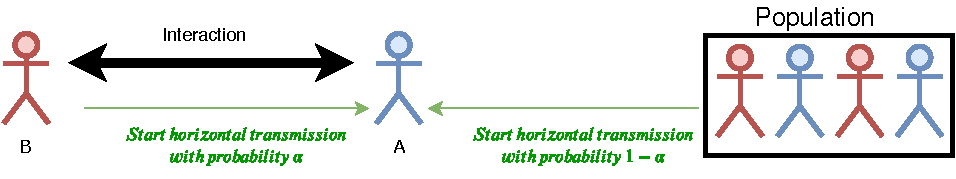
\includegraphics[scale=1]{figure1.pdf}
  \caption{\textbf{Cultural horizontal transmission with assortment.} Transmission occurs between interacting partners with probability $\alpha$ (left) or between two random peers with probability $1-\alpha$, where $\alpha$ is the \emph{social association} parameter.
  }
  \label{fig:horizontal}
\end{figure}


%%% Figure: Boundaries figure - only vertical

\begin{figure}[h]
  \centering       
    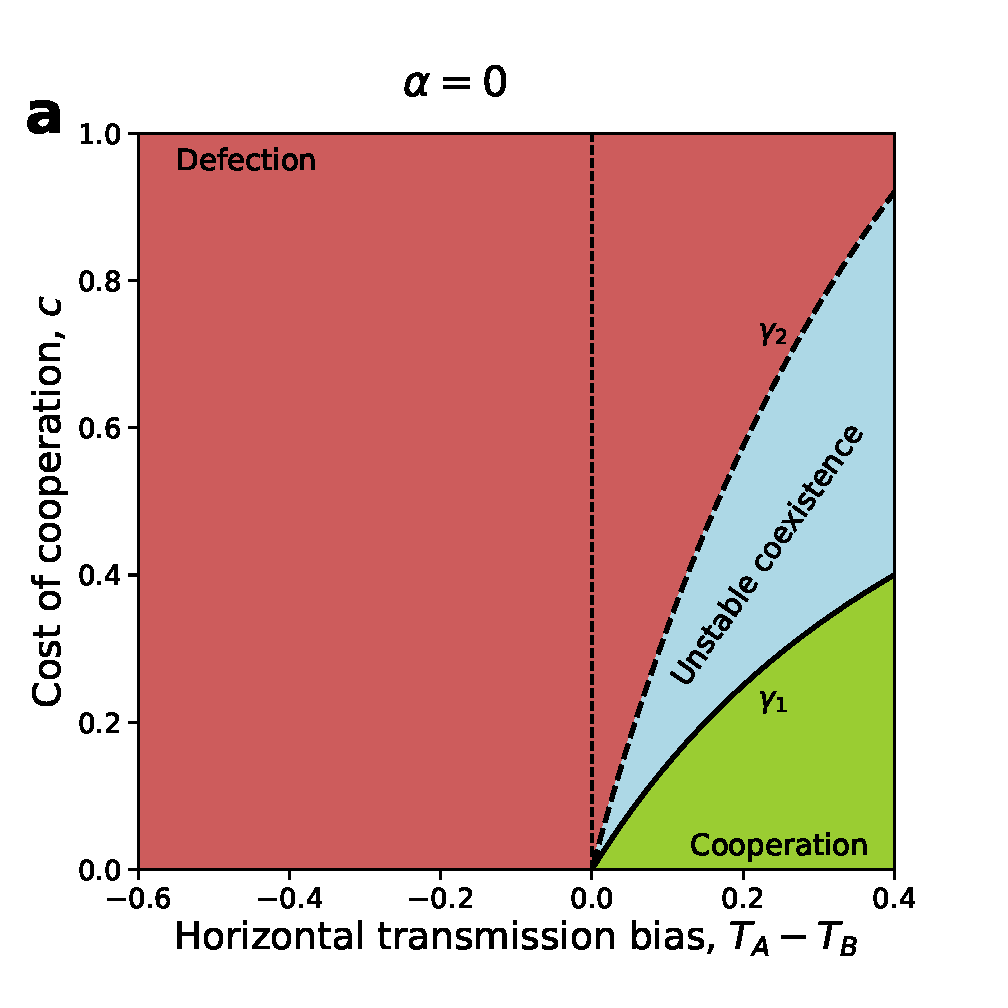
\includegraphics[width=0.45\textwidth]{Result2_c_zero_alpha.eps}
	~
    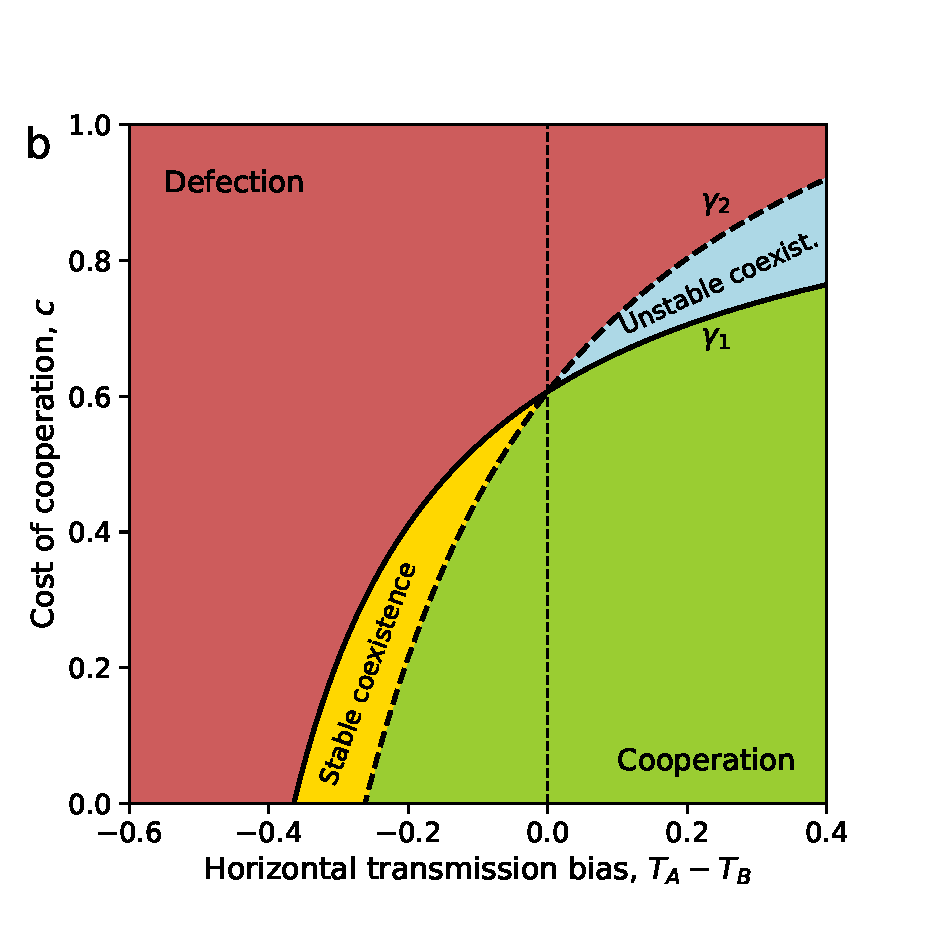
\includegraphics[width=0.45\textwidth]{Result2_c_non_zero_alpha.eps}
    ~
    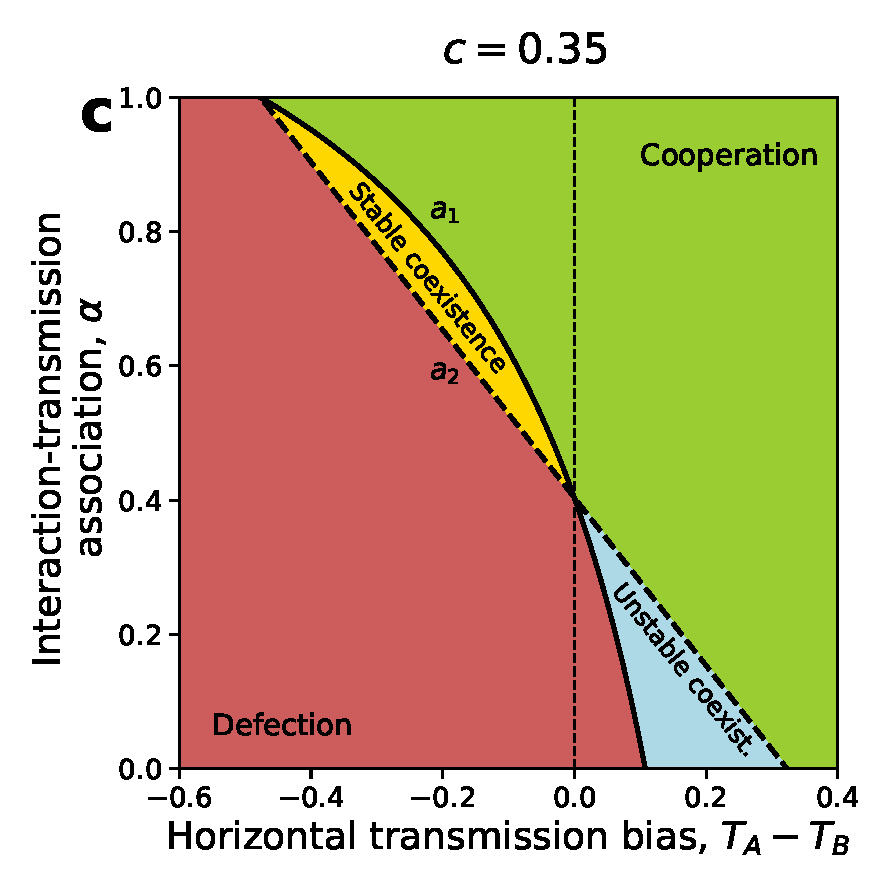
\includegraphics[width=0.45\textwidth]{Result2_alpha.eps}

    \caption{\textbf{Evolution of cooperation under vertical and horizontal cultural transmission.} 
The figure shows the global fixation of cooperation (green), global fixation of defection (red), fixation of either cooperation or defection depending on the initial conditions, i.e. unstable coexistence (blue), and stable coexistence of cooperation and defection (yellow).
In all cases the horizontal bias ($T_A-T_B$) is on the x-axis.
(\textbf{a-b})~The cost of cooperation $c$ is on the y-axis; the cost boundaries $\gamma_1$ and $\gamma_2$ (\autoref{eq:cost_boundaries}) are the solid and dashed lines, respectively. 
(\textbf{c})~social association $\alpha$ is on the y-axis; the social association boundaries $a_1$ and $a_2$ (\autoref{eq:boundries_assortative_meeting}) are the solid and dashed lines, respectively.
Here, $b=1.3$, $T_A=0.4$. (\textbf{a})~$\alpha = 0$.(\textbf{b})~$\alpha = 0.7$. (\textbf{c})~$c = 0.35$.
  	}
    \label{fig:result2}
\end{figure}
%TODO add panel d?



%%% Figure: Boundaries figure - vertical and oblique

\begin{figure}[h]
  \centering       
    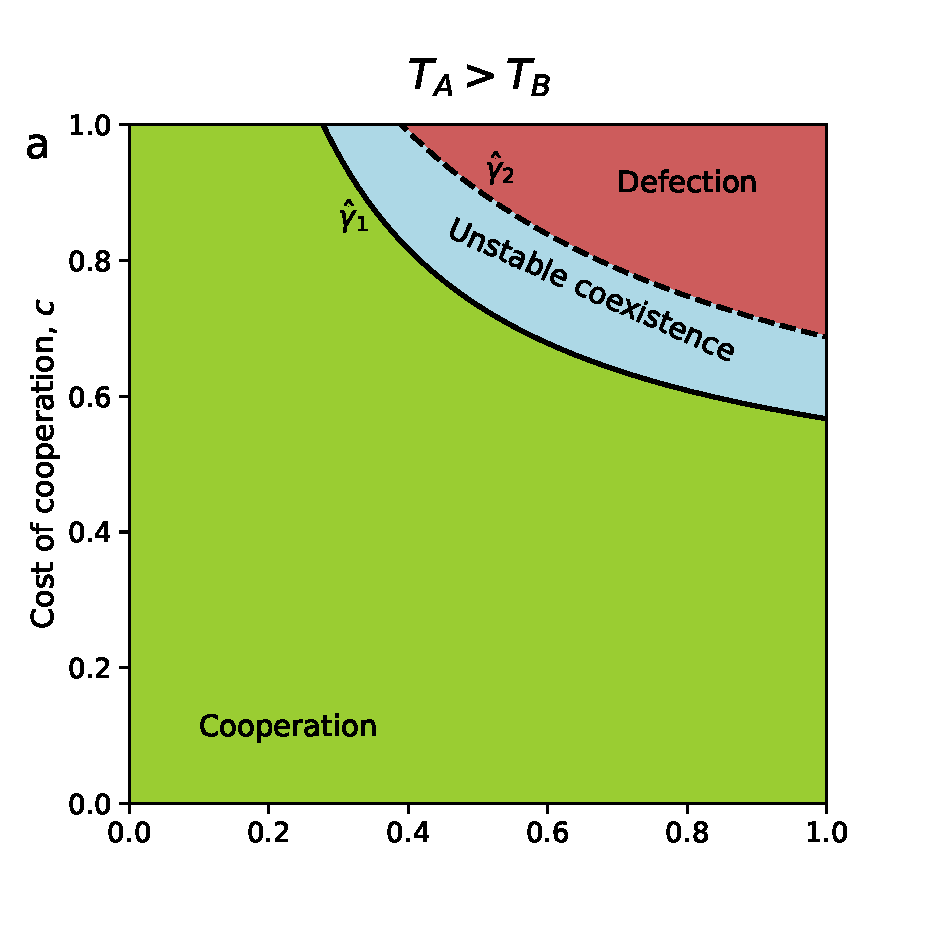
\includegraphics[width=0.45\textwidth]{Result3_TA_TB.eps}~
    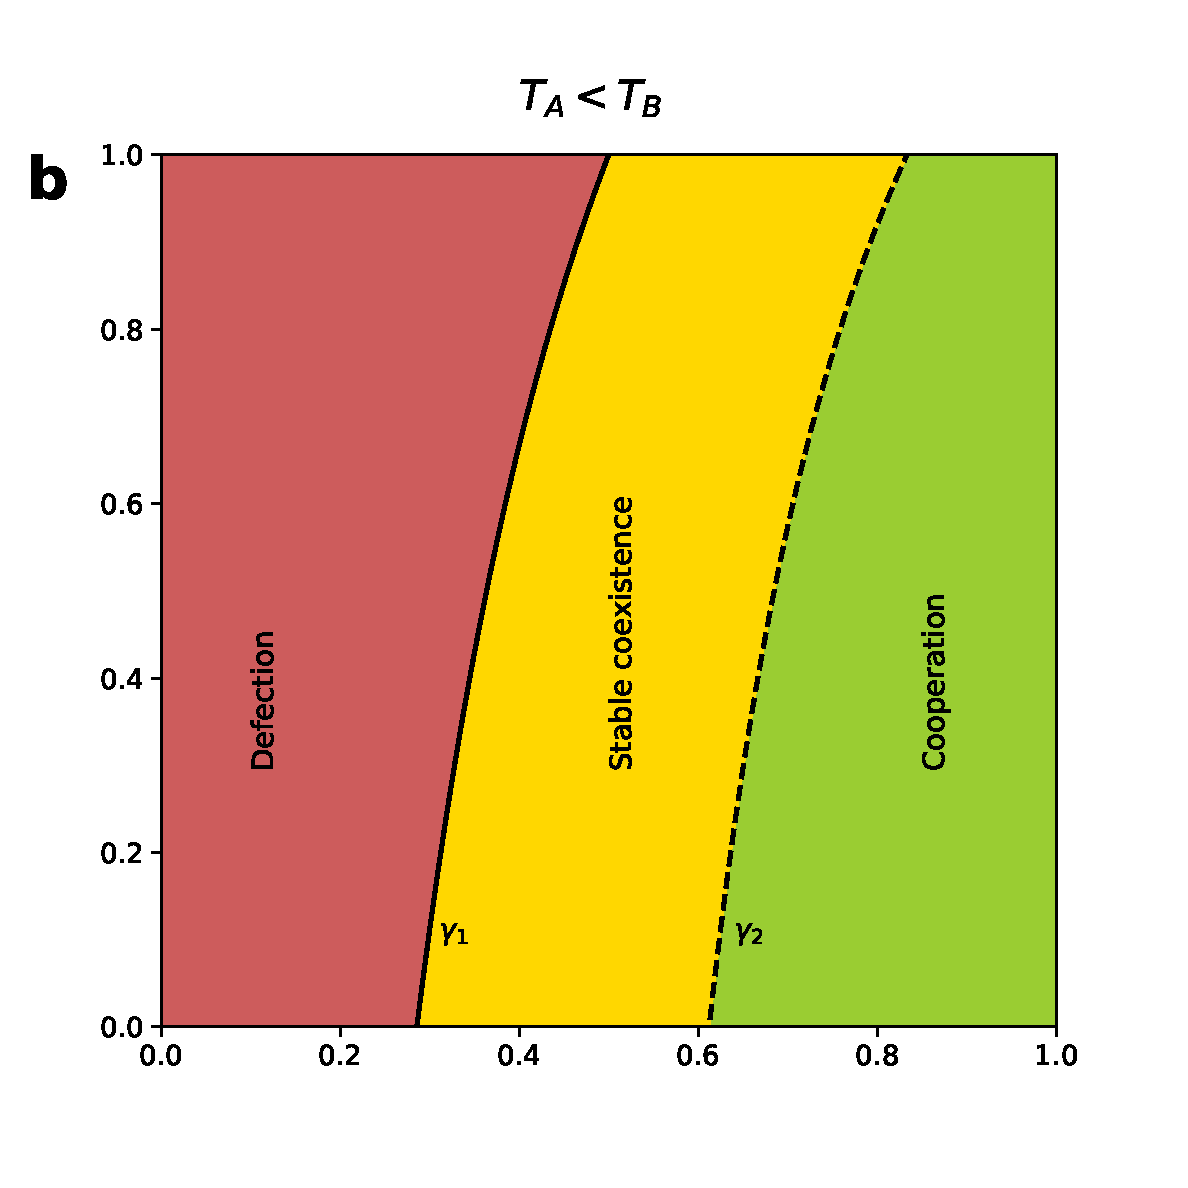
\includegraphics[width=0.45\textwidth]{Result3_TB_TA.eps}
    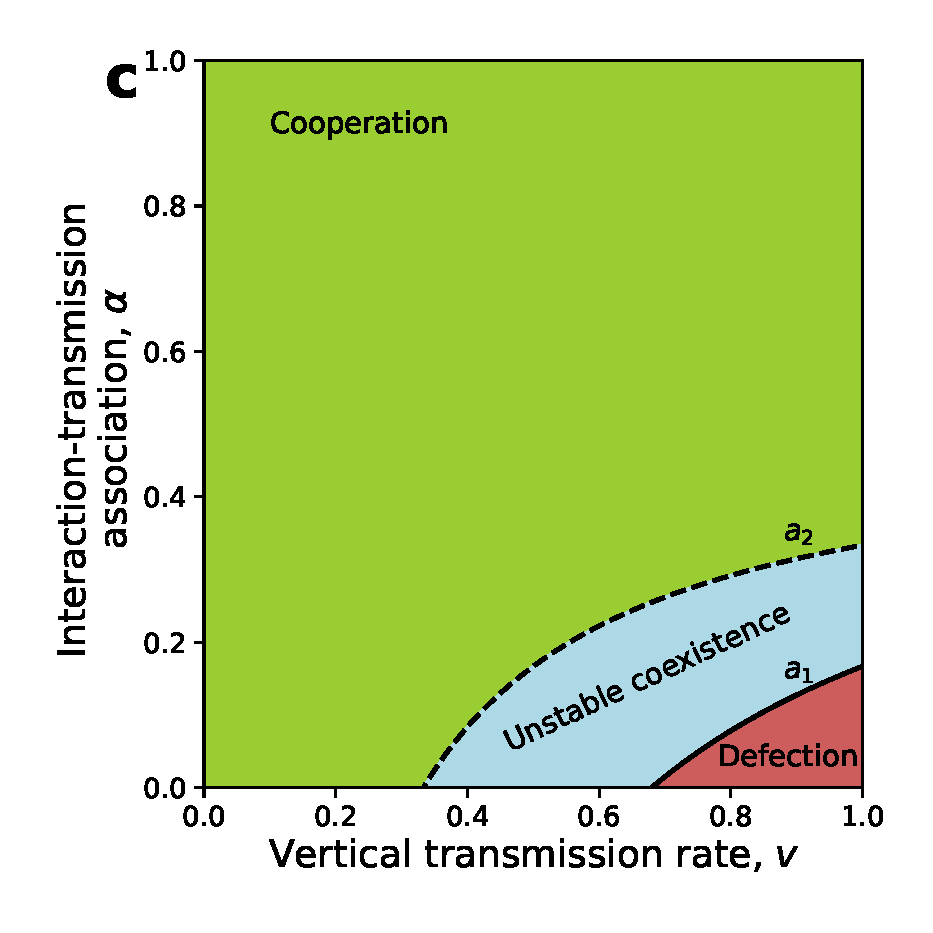
\includegraphics[width=0.45\textwidth]{Result3_alpha_Vs_v_TA_TB.eps}~
    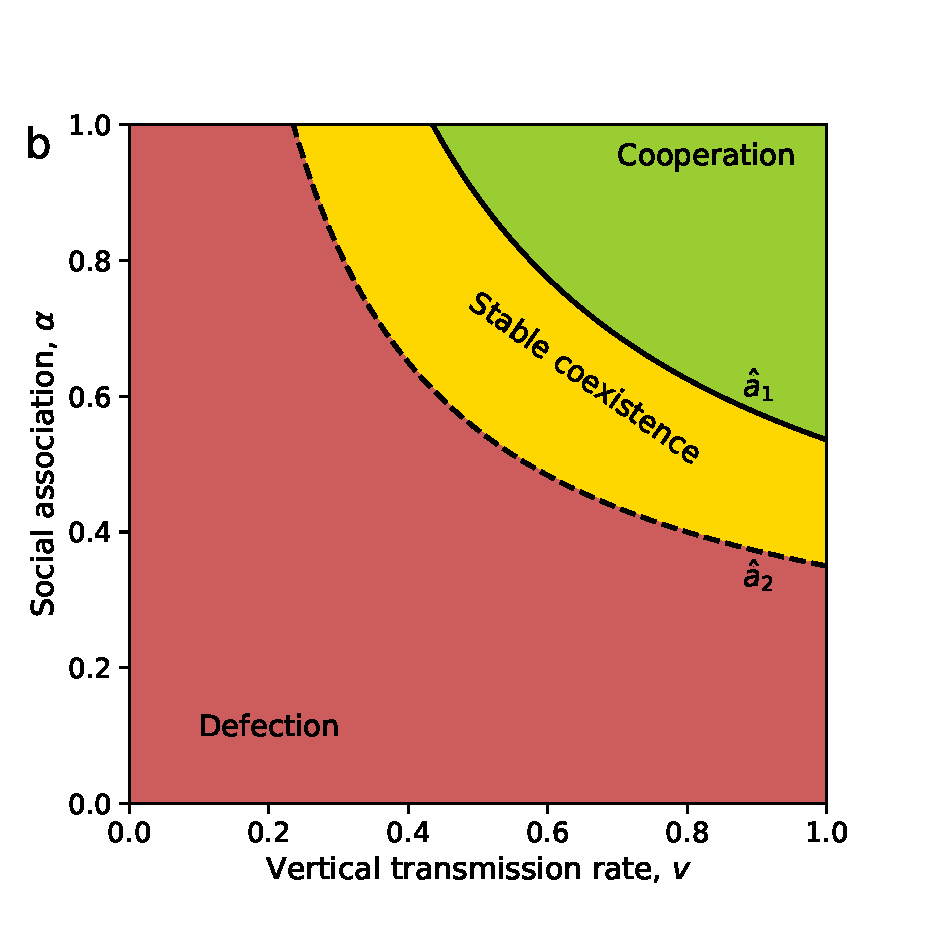
\includegraphics[width=0.45\textwidth]{Result3_alpha_Vs_v_TB_TA.eps}
    \caption{\textbf{Evolution of cooperation under vertical, oblique, and horizontal cultural transmission.} 
    The figure shows the global fixation of cooperation (green), global fixation of defection (red), fixation of either cooperation or defection depending on the initial conditions, i.e. unstable coexistence (blue), and stable coexistence of cooperation and defection (yellow).
	In all cases the vertical transmission rate $v$ is on the x-axis.
	(\textbf{a-b}) The cost of cooperation $c$ is on the y-axis and the cost boundaries $\hat\gamma_1$ and $\hat\gamma_2$ (\autoref{eq:cost_boundaries}) are represented by the solid and dashed lines, respectively. 
    (\textbf{c-d}) The social association $\alpha$ is on the y-axis and the social association boundaries $\hat{a}_1$ and $\hat{a}_2$ (\autoref{eq:boundries_assortative_meeting_general_case}) are represented by the solid and dashed lines, respectively. 
    Horizontal transmission is biased in (\textbf{a,c}) for cooperation, $T_A>T_B$, and in (\textbf{b,d}) for defection, $T_A<T_B$.    
    Here, $T_A = 0.5$, and
    (\textbf{a}) $b=1.2$, , $T_B = 0.4$, $\alpha = 0.4$;
    (\textbf{b}) $b=2$, $T_B = 0.7$, $\alpha = 0.7$;
    (\textbf{c}) $b=1.2$, $T_B = 0.4$, $c=0.5$;
    (\textbf{d}) $b=2$, $T_B = 0.7$, $c=0.5$.
    }
    \label{fig:result3}
\end{figure}



%%% Figure: coexistence map
\begin{figure}[h]
  \centering
    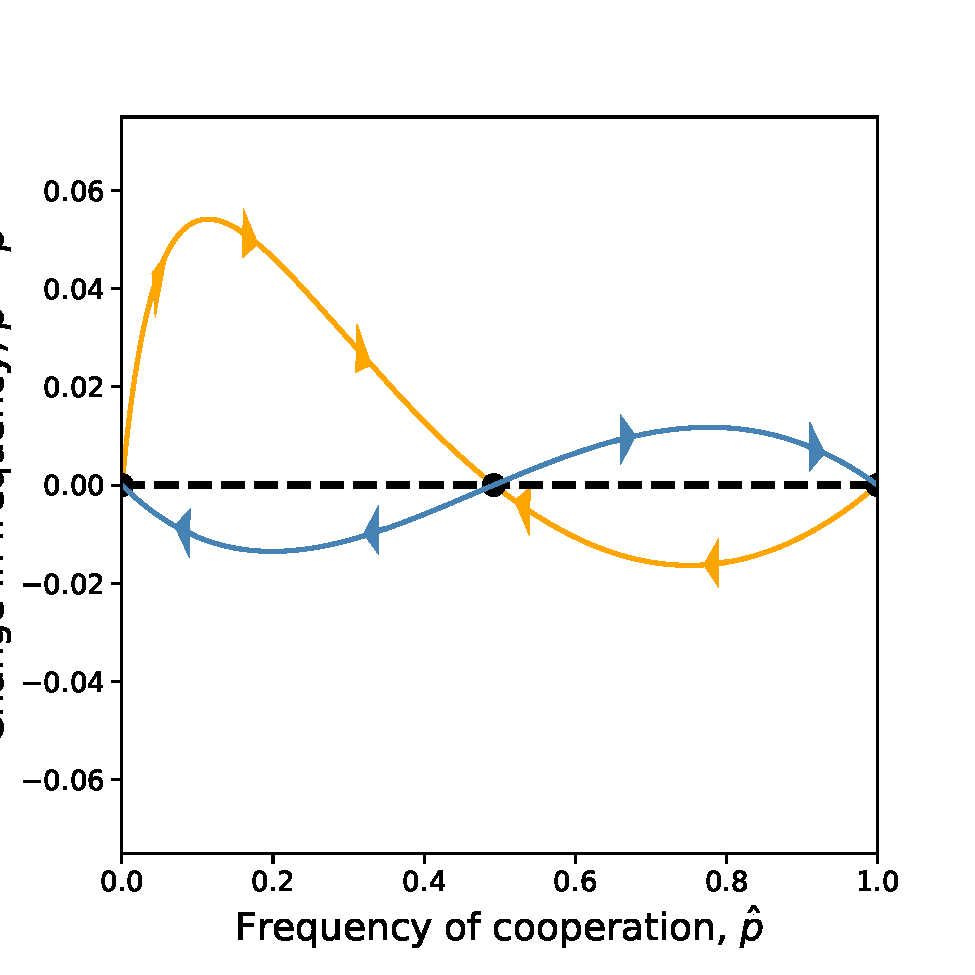
\includegraphics[scale=0.45]{coexistence_without_oblique.pdf}~
    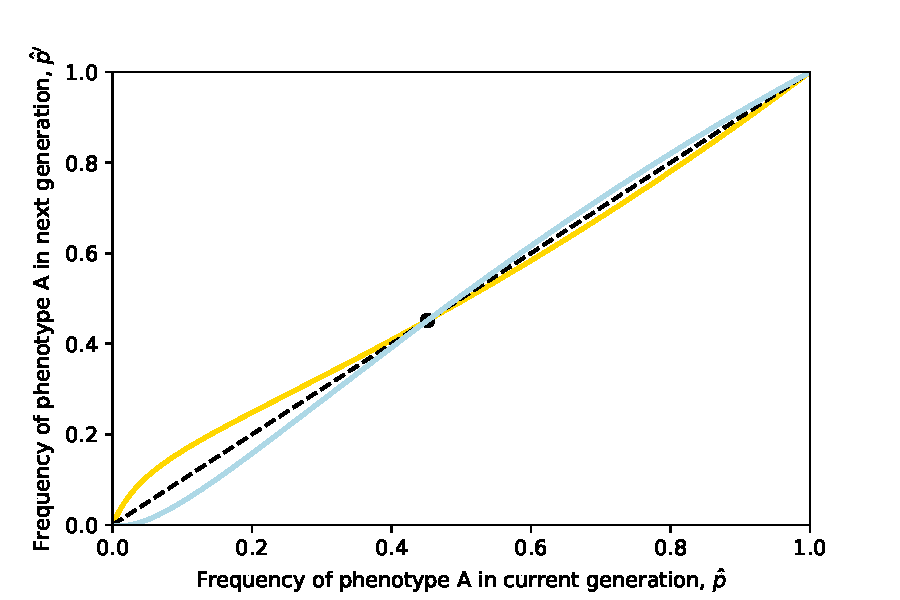
\includegraphics[scale=0.45]{coexistence_with_oblique.pdf}
  \caption{\textbf{Stable and unstable coexistence between cooperation and defection.}
  The curves show the frequency $\hat{p}'$ of the cooperative phenotype $A$ among juveniles in the next generation vs. that in current generation $\hat{p}$ (\autoref{eq:horizontal}).
  The dashed black line is $\hat{p}'=\hat{p}$.
  The curves and the dashed line intersect at the stable equilibrium $\hat{p}^*$ (black circle).
  When $\hat{p} < \hat{p}^*$ the curve is above the dashed line, $\hat{p}' > \hat{p}$, and $\hat{p}$ increases towards $\hat{p}^*$.
  When $\hat{p} > \hat{p}^*$ the curve is below the dashed line, $\hat{p}' < \hat{p}$, and $\hat{p}$ decreases towards $\hat{p}^*$.\\
  \textbf{(a)} There is no oblique transmission, $v=1$.
  The orange curve, for which the polymorphic equilibrium is stable, is given by $T_A = 0.4$, $T_B = 0.9$, $b = 12$, $c=0.35$, and $\alpha = 0.45$, which give $\gamma_2<c<\gamma_1$ (\autoref{eq:cost_boundaries}).
  The blue curve, for which the equilibrium is unstable, is given by $T_A = 0.5$, $T_B = 0.1$, $b = 1.3$, $c=0.904$, and $\alpha = 0.4$, which give $\gamma_1<c<\gamma_2$.\\
  \textbf{(b)} Oblique transmission exists. 
  The orange curve is parameterized by $T_A = 0.4$, $T_B = 0.9$, $b = 20$, $c=0.1$, $\alpha = 1$, and $v=0.4$, which give $0<\beta_3<\beta_1$ (\autoref{eq:polynomial_coefficients}).
  The blue curve is parameterized by $T_A = 0.5$, $T_B = 0.4$, $b=1.2$, $c=0.487$, $\alpha = 0.09$ and $v=0.6$, which give $\beta_1<\beta_3<0$.
  }
  \label{fig:coexistence_recursive}
  \end{figure}



%%% Figure: frequency dynamics
\begin{figure}[h]
  \centering
    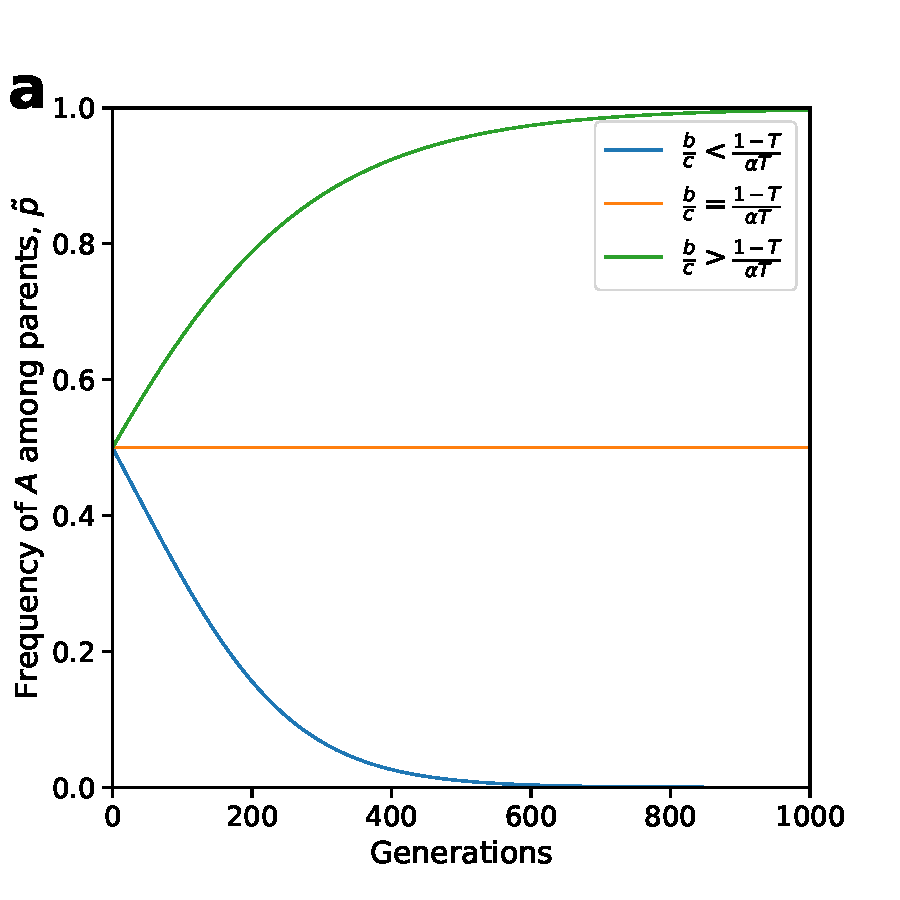
\includegraphics[scale=0.45]{Time_Figure_Equal_Horizontal.pdf}
    ~\\
    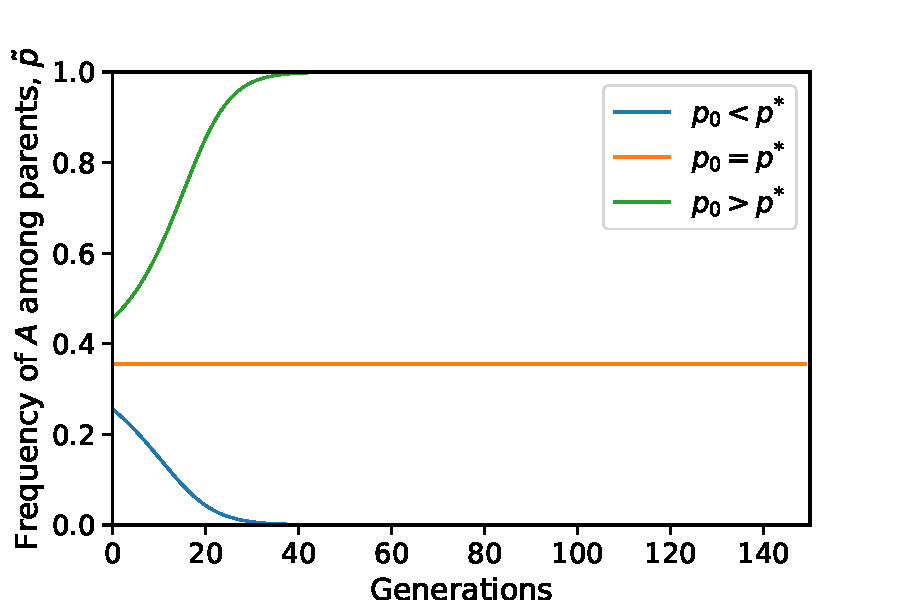
\includegraphics[scale=0.45]{Time_Figure_Only_Vertical_No_Alpha.pdf}
    ~\\
    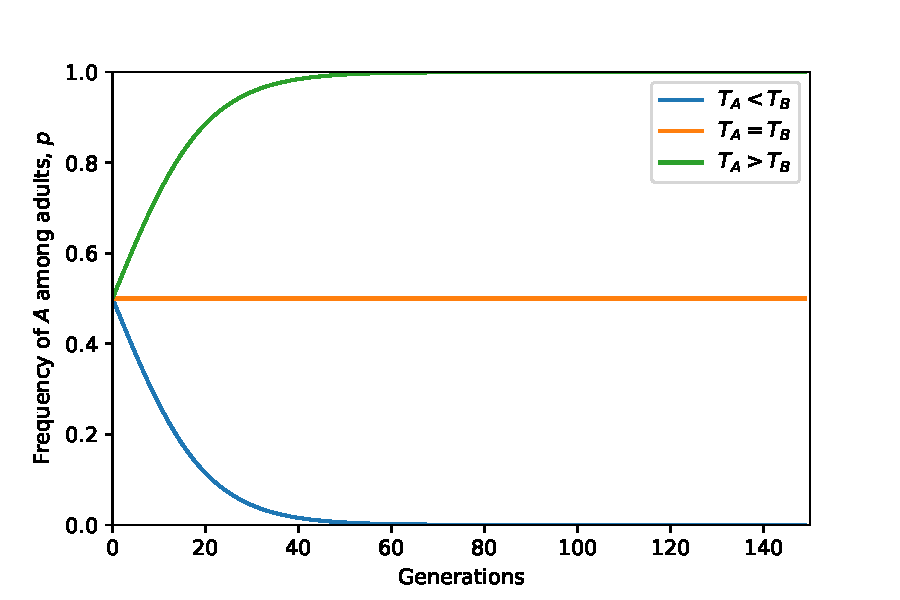
\includegraphics[scale=0.45]{Time_Figure_No_Vertical.pdf}
  \caption{
  \textbf{Dynamics of the frequency of cooperation.}
  The frequency $\tilde{p}$ of parents with cooperative phenotype $A$ in \textbf{(a-b)} and the frequency $p$ of adults with cooperative phenotype $A$ in \textbf{(c)}.
  The different lines correspond to parameter values that lead to fixation of cooperation (green), extinction of cooperation (red), or stable coexistence of cooperators and defectors (yellow).
  \textbf{(a)} $v=1$, $T_A=T_B=T = 0.2$, $\alpha = 0.5 \neq 0$, $\tilde{p}_0 = 0.5$ and $c=0.1$; \textbf{(b)} $v=1$, $\alpha = 0$, $\tilde{p}^* \approx 0.35$, $T_A = 0.65$, $T_B = 0.1$, $b=1.3$ and $c=0.65$; \textbf{(c)} $v=0$, $\alpha =0.5$, $p_0 = 0.5$, $T_A = 0.5$, $b=1.3$ and $c = 0.5$.
  }
  \label{fig:results}
\end{figure}



%%% Figure: Spatial model - global selection
\begin{figure}[h]
  \centering
   \includegraphics[scale=0.5]{{Ta=Tb_b=1.3_globalSelection}.pdf}
    ~
    \includegraphics[scale=0.5]{{Ta=0.4_Tb=0.3-0.5_b=1.3_globalSelection}.pdf} \\
  \caption{
  \textbf{Evolution of cooperation in a spatial model.}
  The expected frequency of cooperators in a structured population after 10,000 generations is shown (red for 0\%, green for 100\%) as function of both the cost of cooperation ($c$) on the y-axis, and the symmetric horizontal transmission rate ($T=T_A=T_B$) on the x-axis of the left panel, or the transmission bias $T_A-T_B$ on the x-axis of the right panel.
  The population evolves on a 100-by-100 grid.
  Cooperation and horizontal transmission are both local between adjacent sites, and each site had 8 neighbors.
  Selection operates globally (see \autoref{fig:spatial_local_selection} for results from a model with local selection).
  The black curves represent the cost boundaries for the evolution of cooperation in a well-mixed population with social association where $\alpha=1/8$ in \textbf{(a)} \autoref{eq:equal_transmission} and \textbf{(b)} \autoref{eq:cost_boundaries}.
  Simulations were stopped at generation 10,000 or if one of the phenotypes fixed and 50 simulations were executed for each parameter set.
  Here, population size is 10,000 (100-by-100 grid), benefit of cooperation, $b=1.3$, perfect vertical transmission $v=1$.
  \textbf{(a)} Symmetric horizontal transmission, $T=T_A=T_B$.
  \textbf{(b)} Horizontal transmission rates $T_A=0.4$, $0.3<T_B<0.5$.
  }
  \label{fig:spatial}
\end{figure}

%%% Figure: Spatial model - local selection
\begin{figure}[h]
  \centering
   \includegraphics[scale=0.5]{{Ta=Tb_b=1.3_localSelection}.pdf}
    ~
    \includegraphics[scale=0.5]{{Ta=0.4_Tb=0.3-0.5_b=1.3_localSelection}.pdf} \\
  \caption{
  \textbf{Evolution of cooperation in a spatial model with local selection.}
  The expected frequency of cooperators in a structured population after 10,000 generations is shown (red for 0\%, green for 100\%) as function of both the cost of cooperation ($c$) on the y-axis, and the symmetric horizontal transmission rate ($T=T_A=T_B$) on the x-axis of the left panel, or the transmission bias $T_A-T_B$ on the x-axis of the right panel.
  The population evolves on a 100-by-100 grid.
  Cooperation and horizontal transmission are both local between adjacent sites, and each site had 8 neighbors.
  Selection operates locally (see \autoref{fig:spatial} for results from a model with global selection).
  The black curves represent the cost boundaries for the evolution of cooperation in a well-mixed population with social association where $\alpha=1/8$ in \textbf{(a)} \autoref{eq:equal_transmission} and \textbf{(b)} \autoref{eq:cost_boundaries}.
  Simulations were stopped at generation 10,000 or if one of the phenotypes fixed and 50 simulations were executed for each parameter set.
  Here, population size is 10,000 (100-by-100 grid), benefit of cooperation, $b=1.3$, perfect vertical transmission $v=1$.
  \textbf{(a)} Symmetric horizontal transmission, $T=T_A=T_B$.
  \textbf{(b)} Horizontal transmission rates $T_A=0.4$, $0.3<T_B<0.5$.
  }
  \label{fig:spatial_local_selection}
\end{figure}

% Fluctuations in spatial model
\begin{figure}[h]
  \centering
   \includegraphics[scale=0.75]{{timeSereis_b=1.3_TA=0.4_TB=0.435_c=0.02_globalSelection_normalizeByNumInteractions}.pdf}
   \caption{
    \textbf{Stable coexistence of both phenotypes in a spatial model.}
    The frequency of cooperators (green) and defectors (red) in a spatial model. 
    Both phenotypes start at 50\% frequency.
    The figure shows that neither phenotype is fixed throughout the simulation, maintaining a stochastic coexistence.
    Here, population size is 10,000 (100-by-100 grid), selection operates globally, 
    benefit and cost of cooperation $b=1.3$ and $c=0.02$, perfect vertical transmission $v=1$, horizontal transmission rates $T_A = 0.4 < T_B = 0.435$.
    }
    \label{fig:spatial_fluctuations}
  \end{figure}
  %TODO: edit this caption. DC

%%%
\end{document}